\section{A uniform transition at outer order one}
\label{eutrans:sec:main}

This section proves the near-critical reversal conjecture
\texttt{research:conj:crossing} in the pinned continuation
\texttt{tetralogarithm-euler-polynomial-zeros} and determines its first
logarithmic correction. The distinction between an expansion for fixed
parameters and an expansion uniform at an integer outer order is essential:
the coefficient of the algebraic density vanishes at outer order one,
while an exponentially small density survives. Both contributions are
of the same size at the reversal.

\subsection{Definitions and the inherited sign theorem}

For $a,b>0$, write
\[
 F_{a,b}(z)=\sum_{n\geq1}\frac{H_{n-1}^{(b)}}{n^a}z^n,
 \qquad H_m^{(b)}=\sum_{j=1}^m j^{-b},
 \qquad g_{a,b}=\operatorname{Im}F_{a,b}(i),
\]
where the boundary value is its analytic continuation. Define
\[
 f_n=\frac{H_{2n}^{(b)}}{(2n+1)^a},\qquad
 d_j=\sum_{n=0}^j(-1)^n\binom jn f_n,\qquad
 E_N=\sum_{j=0}^{N-1}\frac{d_j}{2^{j+1}},\qquad
 R_N(a,b)=2^N(E_N-g_{a,b}).
\]
The axis $a=0$ uses the same analytic convention. The comparison of
interest fixes the total order:
\[
 \mathcal D_{a,b}(N)=R_N(a,b)-R_N(0,a+b).
\]
Set
\begin{align}
 h_b(T)&=\frac1{\Gamma(b)}\int_T^\infty
                    \frac{v^{b-1}}{e^v-1}\,dv,
 & I^ah_b(T)&=\frac1{\Gamma(a)}\int_0^T(T-v)^{a-1}h_b(v)\,dv,
 \label{eutrans:eq:seed}\\
 D_{a,b}(T)&=(I^ah_b)'(T)
              +\frac{T^{a+b-1}}{\Gamma(a+b)(e^T-1)},
 & q(T)&=1-e^{-2T}.
 \label{eutrans:eq:density}
\end{align}
The exact compensated Euler formula yields
\begin{equation}\label{eutrans:eq:interpolation}
 \mathcal D_{a,b}(s)=-\int_0^\infty D_{a,b}(T)
          \frac{e^{-T}q(T)^s}{1+e^{-2T}}\,dT,
 \qquad s\geq1.
\end{equation}
It agrees with the preceding definition at integers and supplies the
real interpolation used below. All its derivatives in $s$ are ordinary
absolutely convergent integrals. In fact, with
$\ell(T)=-\log q(T)>0$,
\begin{equation}\label{eutrans:eq:derivatives}
 (-1)^r\mathcal D_{a,b}^{(r)}(s)
 =-\int_0^\infty D_{a,b}(T)
    \frac{e^{-T}q(T)^s\ell(T)^r}{1+e^{-2T}}\,dT.
\end{equation}

The prior phase theorem \cite{RepoEuler} establishes the following facts. For $0<a<1$,
$D_{a,b}(T)$ has precisely one sign change, from positive to negative.
For every integer $r\geq0$, $\mathcal D_{a,b}^{(r)}$ has one simple
zero $\nu_r(a,b)>1$, and
\[
 1<\nu_0(a,b)<\nu_1(a,b)<\cdots.
\]
The sign of $(-1)^r\mathcal D_{a,b}^{(r)}$ is negative before that
zero and positive afterwards. In particular $\nu_0=\nu$ is the
reversal index, while $\nu_1$ is the location of the unique positive
maximum of $\mathcal D_{a,b}$. These facts can also be checked directly from
\eqref{eutrans:eq:derivatives}: the ratio of the weights at two $s$
values is strictly increasing in $T$, so subtracting its value at the
density crossing proves the one-zero property. A similar comparison
with the strictly decreasing function $\ell(T)$ orders the derivative
zeros. We use this already proved sign theorem to identify the unique
roots isolated by our uniform estimates.

Throughout the uniform statements, $B=[b_-,b_+]$ is any fixed compact
interval in $(0,\infty)$ and $r$ is a fixed nonnegative integer. Put
\[
 a=1-\varepsilon,\qquad
 \lambda=\log(1/\varepsilon),\qquad p=b+1.
\]
Choose $\varepsilon_0<\min(1/2,b_-/2)$. In particular, the parameters
used here are strictly in the finite-measure region $a+b>1$; no
unweighted hypersingular integral is introduced in this joint limit.

\subsection{The reversal asymptotic and its correction}

Define
\begin{align}
 K_{b,r}&=b\Gamma(b+1)\zeta(b+1)
              \frac{\Gamma(r+1/2)}{\Gamma(r+1)},
 \label{eutrans:eq:K}\\
 \delta_{b,r}&=b-\frac b2\psi(r+1)-\frac12\psi(r+1/2)
      -\frac{(b+1)\zeta(b+2)}{2\zeta(b+1)}.
 \label{eutrans:eq:delta}
\end{align}
All zeta values in these constants lie in their absolutely convergent
range, and both gamma factors have positive arguments.

\begin{theorem}[Near-critical reversal and derivative zeros]
\label{eutrans:thm:crossing}
As $\varepsilon\downarrow0$, uniformly for $b\in B$ and each fixed $r$,
\begin{align}
 \frac12\log\nu_r(1-\varepsilon,b)
 ={}&\lambda+p\log\lambda-\log K_{b,r}\notag\\
 &+\frac{p^2\log\lambda-p\log K_{b,r}+\delta_{b,r}}{\lambda}
 +O_{B,r}\left(\frac{(\log\lambda)^2}{\lambda^2}\right).
 \label{eutrans:eq:Lroot}
\end{align}
Equivalently,
\begin{align}
 \nu_r(1-\varepsilon,b)
 ={}&\frac{\lambda^{2b+2}}{K_{b,r}^2\varepsilon^2}
 \Biggl[1+
 \frac{2p^2\log\lambda-2p\log K_{b,r}+2\delta_{b,r}}{\lambda}
 \notag\\
 &\hspace{30mm}+O_{B,r}\left(\frac{(\log\lambda)^2}{\lambda^2}\right)
 \Biggr].
 \label{eutrans:eq:nuroot}
\end{align}
For $r=0$, this proves the proposed leading law
\begin{equation}\label{eutrans:eq:conjecture}
 \nu(1-\varepsilon,b)\sim
 \frac{(\log(1/\varepsilon))^{2b+2}}
 {\pi b^2\Gamma(b+1)^2\zeta(b+1)^2\varepsilon^2}.
\end{equation}
Its first correction uses
\begin{equation}\label{eutrans:eq:delta0}
 \delta_{b,0}=b+\frac{b+1}{2}\gamma+\log2
                   -\frac{(b+1)\zeta(b+2)}{2\zeta(b+1)}.
\end{equation}
\end{theorem}

The $\log\log(1/\varepsilon)/\log(1/\varepsilon)$ correction is
substantial at accessible parameter values. Keeping the implicit
logarithmic equation gives a more useful approximation.

\begin{corollary}[An approximation in terms of Lambert $W$]
\label{eutrans:cor:lambert}
For sufficiently small $\varepsilon$, put
\begin{equation}\label{eutrans:eq:Lambert}
 \widehat L_{b,r}=-p\,W_{-1}\left(
             -\frac{(K_{b,r}\varepsilon)^{1/p}}p\right).
\end{equation}
Here $W_{-1}$ is the real branch with values at most $-1$.
Then $\widehat L_{b,r}>p$ and, uniformly for $b\in B$,
\begin{equation}\label{eutrans:eq:Lambert-correction}
 \frac12\log\nu_r(1-\varepsilon,b)
 =\widehat L_{b,r}+
       \frac{\delta_{b,r}}{\widehat L_{b,r}-p}
       +O_{B,r}(\widehat L_{b,r}^{-2}).
\end{equation}
\end{corollary}

We now prove the theorem with the estimates that control both limits.

\subsection{Preserving the vanishing algebraic amplitude}

The seed moments are
\begin{equation}\label{eutrans:eq:moments}
 m_j(b)=\int_0^\infty v^j h_b(v)\,dv
       =\frac{(b)_{j+1}}{j+1}\zeta(b+j+1).
\end{equation}
Indeed, Tonelli first integrates $v^j$ up to the outer variable, and
then expansion of $(e^v-1)^{-1}$ gives a sum of gamma integrals. In
particular,
\[
 m_0=b\zeta(b+1),\qquad
 m_1=\frac{b(b+1)}2\zeta(b+2).
\]
Every fixed moment is uniformly bounded as $b$ ranges over $B$.

\begin{lemma}[A uniform density estimate with an $\varepsilon$ factor]
\label{eutrans:lem:density}
For some $M$ depending only on $B$, uniformly for $T\geq2$,
$b\in B$, and $0\leq\varepsilon\leq\varepsilon_0$,
\begin{align}
 (I^{1-\varepsilon}h_b)'(T)
 ={}&h_b(T)-\frac{\varepsilon T^{-1-\varepsilon}}
                  {\Gamma(1-\varepsilon)}
       \left[m_0+\frac{(1+\varepsilon)m_1}{T}
                    +O_B(T^{-2})\right]\notag\\
 &+O_B\left(\varepsilon e^{-T/2}(1+T)^M\right).
 \label{eutrans:eq:uniform-density}
\end{align}
Moreover,
\begin{equation}\label{eutrans:eq:h-infty}
 h_b(T)=\frac{e^{-T}T^{b-1}}{\Gamma(b)}
                   \{1+O_B(T^{-1})\}.
\end{equation}
The $O_B(T^{-2})$ term in \eqref{eutrans:eq:uniform-density} is
inside the bracket multiplied by $\varepsilon$.
\end{lemma}

\begin{proof}
For $T>0$, the regularized differentiation formula is
\begin{equation}\label{eutrans:eq:Marchaud}
 (I^{1-\varepsilon}h_b)'(T)
 =\frac1{\Gamma(1-\varepsilon)}\left[
 T^{-\varepsilon}h_b(T)
 +\varepsilon\int_0^T
       \frac{h_b(T)-h_b(v)}{(T-v)^{1+\varepsilon}}\,dv\right].
\end{equation}
The integral is absolutely convergent. At $v=0$, $h_b(v)$ is
locally integrable; at $v=T$, the numerator is $O(T-v)$ and
$\varepsilon<1$. One way to derive the identity without using an
endpoint value $h_b(0)$ is to replace the fractional kernel by
$(T-v+\eta)^{-\varepsilon}$, differentiate, subtract $h_b(T)$ in
the differentiated integral, and let $\eta\downarrow0$. Dominated
convergence applies to the subtracted integral and to the original
fractional integral on compact positive $T$ intervals. Its boundary
term tends to $T^{-\varepsilon}h_b(T)$. The same computation at
$\varepsilon=0$ gives $(I^1h_b)'=h_b$.

Split the integral in \eqref{eutrans:eq:Marchaud} at $v=T/2$.
On the first part retain $-h_b(v)$ and expand
\[
 (T-v)^{-1-\varepsilon}=T^{-1-\varepsilon}
 \left[1+(1+\varepsilon)\frac vT
                  +O\left(\frac{v^2}{T^2}\right)\right].
\]
The Taylor bound is uniform for $0\leq v/T\leq1/2$ and the chosen
compact $\varepsilon$ interval. Replacing the truncated moments by
the full moments changes the result by an exponential error, since
$h_b(v)$ decays exponentially at infinity with a uniform polynomial
bound. The second moment bounds the Taylor remainder and yields
the bracket in \eqref{eutrans:eq:uniform-density}.

Here are bounds for the remaining terms. For $u\geq1$,
\[
 |h_b(u)|+|h_b'(u)|
       \leq C_B e^{-u}(1+u)^{M_0}.
\]
For $v\geq T/2$, the mean value theorem gives
\[
 |h_b(T)-h_b(v)|
 \leq C_B e^{-T/2}(1+T)^{M_0}\min(T-v,1).
\]
Consequently its integral against $(T-v)^{-1-\varepsilon}$ is at
most $C_Be^{-T/2}(1+T)^{M_0+1}$, uniformly in $\varepsilon$:
the integral on $0<T-v<1$ is bounded by $(1-\varepsilon_0)^{-1}$,
and the rest by $1+\log T$.
The $h_b(T)$ contribution on $v<T/2$ satisfies the same type of
bound. Finally
\[
 \left|\frac{T^{-\varepsilon}}{\Gamma(1-\varepsilon)}-1\right|
                \leq C\varepsilon(1+\log T),
\]
by the mean value theorem in $\varepsilon$. Multiplication by
$h_b(T)$ absorbs this discrepancy in the exponential error. Every
discarded term in this paragraph carries the prefactor
$\varepsilon$ from \eqref{eutrans:eq:Marchaud}, or the same factor
from the last inequality. Increasing $M$ proves
\eqref{eutrans:eq:uniform-density}.

For \eqref{eutrans:eq:h-infty}, expand the Bose denominator as
$e^{-v}\{1+O(e^{-v})\}$. In the leading integral set $v=T+u$,
factor $e^{-T}T^{b-1}$, and use
$(1+u/T)^{b-1}=1+O_B(u(1+u)^{M_1}/T)$ inside its exponential
integral. This proves the estimate uniformly on $B$.
\end{proof}

\subsection{A joint expansion under the Euler kernel}

Put
\begin{align}
 A_{b,r}&=\frac{m_0(b)\Gamma(r+1/2)}2,
 & B_{b,r}&=\frac{\Gamma(r+1)}{2\Gamma(b+1)},
 \label{eutrans:eq:AB}\\
 \alpha_{b,r}&=\frac12\psi(r+1/2)+\frac{m_1(b)}{m_0(b)},
 & \beta_{b,r}&=b-\frac b2\psi(r+1).
 \label{eutrans:eq:alphabeta}
\end{align}
Thus $K_{b,r}=A_{b,r}/B_{b,r}$ and
$\delta_{b,r}=\beta_{b,r}-\alpha_{b,r}$.

\begin{lemma}[Uniform competition of two scales]
\label{eutrans:lem:joint}
Let $L=\tfrac12\log s$ and $\lambda=\log(1/\varepsilon)$. Uniformly
for $b\in B$ and $\lambda/2\leq L\leq2\lambda$, as
$\varepsilon\downarrow0$,
\begin{align}
 (-1)^r\mathcal D_{1-\varepsilon,b}^{(r)}(s)
 ={}&\varepsilon A_{b,r}s^{-r-1/2}L^{-1}
       \{1+\alpha_{b,r}/L+O_{B,r}(L^{-2})\}\notag\\
 &-B_{b,r}s^{-r-1}L^b
       \{1+\beta_{b,r}/L+O_{B,r}(L^{-2})\}.
 \label{eutrans:eq:joint}
\end{align}
The two remainder terms are bounded separately by their respective
displayed scales. In particular the estimate remains useful where
the leading terms cancel.
\end{lemma}

\begin{proof}
Insert Lemma~\ref{eutrans:lem:density} into
\eqref{eutrans:eq:density} and \eqref{eutrans:eq:derivatives}. The
change of variable $t=\sqrt{s}e^{-T}$ gives $T=L-\log t$ and
$e^{-T}\,dT=-s^{-1/2}\,dt$. On the central interval
$s^{-1/4}\leq t\leq s^{1/4}$ one has $T\in[L/2,3L/2]$ and
\begin{align*}
 \frac{(1-t^2/s)^s}{1+t^2/s}&\longrightarrow e^{-t^2},\\
 \{s[-\log(1-t^2/s)]\}^r&\longrightarrow t^{2r}.
\end{align*}
Their differences from the limits have integrals bounded by
$O_r(s^{-1})$ times fixed Gaussian moments. For example, when
$t^2/s\leq1/2$,
\[
 \left|\frac{(1-t^2/s)^s}{1+t^2/s}-e^{-t^2}\right|
 \leq C s^{-1}e^{-t^2}(t^2+t^4),
\]
and the second replacement has an analogous bound with a further
fixed polynomial in $t$. The powers of $T$ remain comparable to
their powers of $L$ on this central interval.

The tails require no uniformity assumption beyond the stated window.
For $T<L/2$, use $q(T)^s\leq\exp(-s e^{-2T})\leq\exp(-e^L)$.
The local bounds can be made explicit: for $0<T\leq1$,
\[
 |D_{1-\varepsilon,b}(T)|\leq C_B
 \bigl(T^{-\varepsilon_0}+T^{b_--1-\varepsilon_0}\bigr)
                                  (1+|\log T|).
\]
Indeed $h_b(T)\leq C_B(1+T^{b_--1})(1+|\log T|)$ follows by
splitting its integral at one; insertion in the compensated
derivative formula, or its beta-integral form
\eqref{eutrans:eq:numerical-density}, gives the displayed estimate.
Since $\varepsilon_0<b_-/2$ and $\varepsilon_0<1/2$, it is
integrable even after multiplication by the additional fixed powers
of $\log T$ coming from $\ell(T)^r$. For $T\geq1$ the density lemma
gives a common polynomial bound. This entire contribution is smaller
than either displayed scale times every power of $L^{-1}$; the
window implies $e^{-2L}\leq\varepsilon\leq e^{-L/2}$.
For $T>3L/2$, equivalently $0<t<s^{-1/4}$, each algebraic contribution
retains its factor $\varepsilon$ and is bounded by the elementary
moments of $t^{2r}$ over this shrinking interval. Exponential
contributions have the extra factor $t$ and are bounded still more
strongly. Logarithmic factors are harmless, since all fixed moments
of $t^c|\log t|^j$ at zero are finite for $c>-1$.

For clarity, the exponential error in
\eqref{eutrans:eq:uniform-density} contributes at most
\[
 O_{B,r}\left(\varepsilon s^{-r-3/4}(1+L)^M\right).
\]
Its ratio to the algebraic scale is
$O_{B,r}(s^{-1/4}(1+L)^{M+1})$, which is smaller than $L^{-2}$
uniformly in the window. The $O(e^{-2T})$ terms produced by the
Bose denominator are likewise negligible relative to the appropriate
exponential scale. These estimates explain why simply deleting an
exponential density in the fixed-parameter expansion would be invalid.

It remains to compute the first corrections. Uniformly in the window,
$\varepsilon\log L=o(L^{-k})$ for every fixed $k$.
Thus $L^{-\varepsilon}$, $\Gamma(1-\varepsilon)^{-1}$, and
$\Gamma(b+1-\varepsilon)^{-1}$ may be replaced by their values at
$\varepsilon=0$ at the required relative accuracy. For any exponent
$c$ in a fixed compact real set, Taylor's theorem on
$|\log t|\leq L/2$ gives
\[
 (L-\log t)^c=L^c\left[
         1-\frac{c\log t}{L}
          +O\left(\frac{(\log t)^2}{L^2}\right)\right].
\]
The full moments needed after extending the central interval are
\begin{align*}
 \int_0^\infty t^{2r}e^{-t^2}\,dt&=\frac12\Gamma(r+1/2),
 &\frac{\int_0^\infty t^{2r}e^{-t^2}\log t\,dt}
       {\int_0^\infty t^{2r}e^{-t^2}\,dt}
       &=\frac12\psi(r+1/2),\\
 \int_0^\infty t^{2r+1}e^{-t^2}\,dt&=\frac12\Gamma(r+1),
 &\frac{\int_0^\infty t^{2r+1}e^{-t^2}\log t\,dt}
       {\int_0^\infty t^{2r+1}e^{-t^2}\,dt}
       &=\frac12\psi(r+1).
\end{align*}
The algebraic density consequently gives $A_{b,r}$ and
$\alpha_{b,r}$. The dominant positive density
$e^{-T}T^b/\Gamma(b+1)$ gives the correction
$-b\psi(r+1)/2$; the retained seed $h_b(T)$ gives the additional
$b/L$, because $\Gamma(b+1)/\Gamma(b)=b$. Hence its coefficient is
$\beta_{b,r}$. The separately bounded second logarithmic moments
prove both remainders in \eqref{eutrans:eq:joint}.
\end{proof}

\subsection{Locating and expanding the unique zero}

\begin{proof}[Proof of Theorem~\ref{eutrans:thm:crossing}]
Define
\[
 S_{\varepsilon,b,r}=
        \frac{\lambda^{2p}}{K_{b,r}^2\varepsilon^2}.
\]
For $s=xS_{\varepsilon,b,r}$ and $x$ in any fixed compact interval
of $(0,\infty)$, $L=\lambda+p\log\lambda-\log K_{b,r}
+\tfrac12\log x$, so $L/\lambda\to1$ uniformly for $b\in B$.
In \eqref{eutrans:eq:joint}, the ratio of the first positive scale
to the second positive scale is
\[
 \varepsilon K_{b,r}\sqrt{s}\,L^{-p}
                =\sqrt{x}(\lambda/L)^p\longrightarrow\sqrt{x}.
\]
Thus the comparison has opposite signs at any fixed $x<1$ and
fixed $x>1$, uniformly for $b\in B$. The inherited uniqueness
theorem identifies its zero and proves
\[
 \nu_r(1-\varepsilon,b)/S_{\varepsilon,b,r}\longrightarrow1.
\]
This first localization justifies using the same window at the zero;
the window has not been assumed as an unproved property of $\nu_r$.

At the zero set $L_r=\tfrac12\log\nu_r$. Equating the two terms
of \eqref{eutrans:eq:joint} and dividing their positive factors gives
\[
 \varepsilon K_{b,r}e^{L_r}L_r^{-p}
       =1+\frac{\delta_{b,r}}{L_r}+O_{B,r}(L_r^{-2}).
\]
Taking logarithms yields the uniform equation
\begin{equation}\label{eutrans:eq:root-equation}
 L_r=\lambda+p\log L_r-\log K_{b,r}
                +\frac{\delta_{b,r}}{L_r}+O_{B,r}(L_r^{-2}).
\end{equation}
First $L_r=\lambda+O_B(\log\lambda)$, and substitution once more
gives $L_r=\lambda+p\log\lambda-\log K_{b,r}
+O_{B,r}(\log\lambda/\lambda)$. Expand $\log L_r$ about
$\lambda$ in \eqref{eutrans:eq:root-equation}. The result is
\eqref{eutrans:eq:Lroot}; Taylor's remainder is
$O_{B,r}((\log\lambda)^2/\lambda^2)$. Exponentiating gives
\eqref{eutrans:eq:nuroot}. The cases $r=0$ follow from
$\Gamma(1/2)=\sqrt\pi$, $\psi(1)=-\gamma$, and
$\psi(1/2)=-\gamma-2\log2$.
\end{proof}

\begin{proof}[Proof of Corollary~\ref{eutrans:cor:lambert}]
The number $\widehat L=\widehat L_{b,r}$ in
\eqref{eutrans:eq:Lambert} is the large solution of
\[
 \widehat L-p\log\widehat L=\lambda-\log K_{b,r}.
\]
It satisfies $\widehat L\sim\lambda$, uniformly on $B$.
On that range the derivative of $L-p\log L$ is
$1-p/L$, bounded away from zero. Comparing with
\eqref{eutrans:eq:root-equation} first gives
$L_r-\widehat L=O_{B,r}(\widehat L^{-1})$. One Taylor expansion
then gives
\[
 (1-p/\widehat L)(L_r-\widehat L)
     =\delta_{b,r}/\widehat L+O_{B,r}(\widehat L^{-2}),
\]
which proves \eqref{eutrans:eq:Lambert-correction}.
\end{proof}

\subsection{A universal profile and the positive maximum}

For $r=0$, abbreviate $K_b=K_{b,0}$ and set
\begin{equation}\label{eutrans:eq:profile-scales}
 S_{\varepsilon,b}=\frac{\lambda^{2b+2}}{K_b^2\varepsilon^2},
 \qquad
 M_{\varepsilon,b}=\frac{\pi b^2\Gamma(b+1)\zeta(b+1)^2}{2}
                  \frac{\varepsilon^2}{\lambda^{b+2}}.
\end{equation}

\begin{theorem}[Universal profile and derivative-root ratios]
\label{eutrans:thm:profile}
For every compact $X\subset(0,\infty)$ and every fixed nonnegative
integer $m$,
\begin{equation}\label{eutrans:eq:profile}
 \frac{\mathcal D_{1-\varepsilon,b}(S_{\varepsilon,b}x)}
             {M_{\varepsilon,b}}
       \longrightarrow x^{-1/2}-x^{-1}
       \qquad\hbox{in }C^m(X),
\end{equation}
uniformly for $b\in B$. Consequently, for every fixed $r$,
\begin{equation}\label{eutrans:eq:root-ratios}
 \frac{\nu_r(1-\varepsilon,b)}{\nu_0(1-\varepsilon,b)}
       \longrightarrow
       \left\{\frac{\sqrt\pi\Gamma(r+1)}{\Gamma(r+1/2)}\right\}^2
       =\left\{\frac{4^r}{\binom{2r}{r}}\right\}^2.
\end{equation}
In particular the maximum is attained at an index asymptotic to
$4\nu_0$, and its height satisfies
\begin{equation}\label{eutrans:eq:height}
 \max_{s\geq1}\mathcal D_{1-\varepsilon,b}(s)
 \sim \frac{\pi b^2\Gamma(b+1)\zeta(b+1)^2}{8}
                  \frac{\varepsilon^2}{\lambda^{b+2}}.
\end{equation}
The same height asymptotic holds when the maximum is restricted to
integer truncation orders. Any maximizing integer is one of the two
integers adjacent to $\nu_1$. The first integer with a strictly
positive comparison is $\lfloor\nu_0\rfloor+1$ and therefore has
the same asymptotic as \eqref{eutrans:eq:conjecture}.
\end{theorem}

\begin{figure}[tbp]
\centering
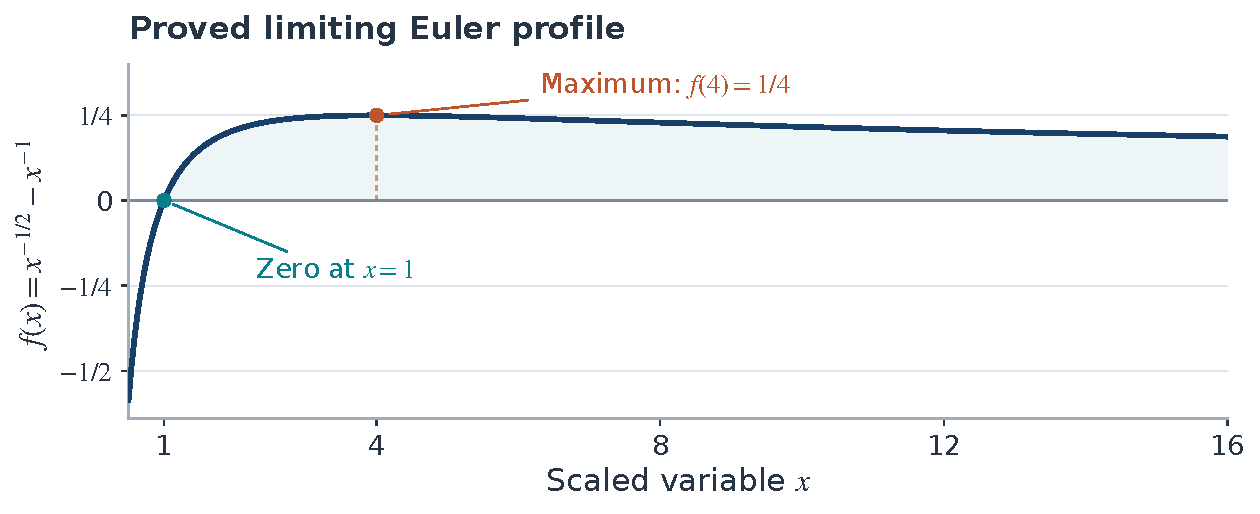
\includegraphics[width=0.90\textwidth]{figures/euler_limiting_profile.pdf}
\caption{The proved limiting profile $x^{-1/2}-x^{-1}$ from
Theorem~\ref{eutrans:thm:profile}, shown for $1/2\leq x\leq16$.
Its zero at one locates the reversal scale and its maximum at four
locates the later positive maximum. This is the limiting function,
not a finite-$\varepsilon$ numerical comparison.}
\label{fig:euler-profile}
\end{figure}

\begin{proof}
The two scales in \eqref{eutrans:eq:joint}, evaluated at
$s=S_{\varepsilon,b}x$, both equal $M_{\varepsilon,b}$ at $x=1$
to leading order. Their $x$ powers are $x^{-1/2}$ and $x^{-1}$.
For every $r\leq m$, the already justified differentiated integral
in Lemma~\ref{eutrans:lem:joint} gives
\[
 \frac{S_{\varepsilon,b}^r
             \mathcal D_{1-\varepsilon,b}^{(r)}
                        (S_{\varepsilon,b}x)}{M_{\varepsilon,b}}
 \longrightarrow(-1)^r\left[
     (1/2)_r x^{-r-1/2}-r!x^{-r-1}\right]
\]
uniformly on $X$. This proves $C^m$ convergence directly, rather than
by differentiating an undifferentiated asymptotic. The root ratios
follow either from these limiting derivatives and uniqueness or
from \eqref{eutrans:eq:nuroot}. The gamma duplication formula gives
the central-binomial expression.

The limiting profile has its unique positive maximum at $x=4$, with
value $1/4$. The inherited global one-maximum theorem places the
actual maximum at $\nu_1$, and \eqref{eutrans:eq:root-ratios} puts
$\nu_1/S_{\varepsilon,b}\to4$. Evaluation of the uniform profile
there gives \eqref{eutrans:eq:height}. No global maximum is inferred
solely from convergence on compact $x$ intervals.
Strict increase before $\nu_1$ and strict decrease afterwards reduce
the integer maximum to the adjacent integers; their rescaled
locations tend to four as well. The asserted first positive integer
follows from the strict sign classification at $\nu_0$.
\end{proof}

\subsection{Verification, integration status, and further questions}

The numerical verifier evaluates the exact density through the
cancellation-free identity
\begin{align}\label{eutrans:eq:numerical-density}
 D_{1-\varepsilon,b}(T)
 ={}&\frac{T^{-\varepsilon}}{\Gamma(1-\varepsilon)}
  \left[h_b(T)-\frac1{\Gamma(b)}\int_0^T
   \frac{v^{b-1}\bigl\{(1-v/T)^{-\varepsilon}-1\bigr\}}
        {e^v-1}\,dv\right]\notag\\
 &+\frac{T^{b-\varepsilon}}{\Gamma(b+1-\varepsilon)(e^T-1)}.
\end{align}
It uses \texttt{expm1} and \texttt{log1p} for the small numerator.
This expression follows by interchanging integrals in $I^ah_b$
before differentiation and is independent of the truncated large-$T$
expansion used in the proof. At $b=1$ it uses
$h_1(T)=-\log(1-e^{-T})$; at $b=2$ it uses
$h_2(T)=\operatorname{Li}_2(e^{-T})-T\log(1-e^{-T})$.
The outer integral is evaluated after the exact Gaussian change of
variables. The output checks $r=0,1,2$, several small values of
$\varepsilon$, and a tighter-tolerance repeat. These values are
floating-point diagnostics, not certified enclosures or proof premises.

\begin{table}[tbp]
\centering\small
\begin{tabular}{rrrr}
\hline
$b$ & $\varepsilon$ & $\tfrac12\log\nu_0$ (quadrature)
 & Error of \eqref{eutrans:eq:Lambert-correction}\\
\hline
1 & $10^{-6}$  & $18.6740498534$ & $-9.5251\,10^{-3}$\\
1 & $10^{-12}$ & $33.6353818511$ & $-2.7315\,10^{-3}$\\
1 & $10^{-24}$ & $62.4857641121$ & $-7.6396\,10^{-4}$\\
2 & $10^{-6}$  & $20.8878708711$ & $-1.0288\,10^{-2}$\\
2 & $10^{-12}$ & $36.3240064653$ & $-2.9060\,10^{-3}$\\
2 & $10^{-24}$ & $65.7078545360$ & $-8.1393\,10^{-4}$\\
\hline
\end{tabular}
\caption{Direct exact-kernel quadrature and the Lambert approximation
for $r=0$. The last column is the numerical value minus the explicit
approximation with its $O(\widehat L^{-2})$ term omitted. These are
numerical diagnostics. The asymptotic theorem does not attach an
effective finite-$\varepsilon$ bound to this column.}
\label{eutrans:tab:diagnostics}
\end{table}

The named conjecture \texttt{research:conj:crossing} can now be
promoted to a theorem, with \eqref{eutrans:eq:nuroot} as a stronger
replacement. The source's fixed-parameter fractional theorem and
one-crossing theorem remain valid; the present result supplies the
missing uniform estimate. Its role is specifically the joint regime
$a\uparrow1$, $s\to\infty$. The compactness condition on $b$ is part
of the theorem. It does not cover $b\downarrow0$, $b\to\infty$, or
derivative orders $r$ growing with $\lambda$.

Several next questions are now concrete. First, expand the bracket in
\eqref{eutrans:eq:uniform-density} to arbitrary order and retain enough
terms of $h_b$ to obtain a full uniform logarithmic expansion of
$\nu_r$. Its coefficients should be expressible through seed zeta
moments and polygamma values at $r+1/2$ and $r+1$; the displayed
proof identifies the required coefficient-generating operations.
Second, derive explicit finite constants in the two separate
remainders of \eqref{eutrans:eq:joint}, so that the Lambert approximation
becomes a practical certified locator. Third, study the simultaneous
limit $r\to\infty$, $\varepsilon\downarrow0$. The fixed-$r$ ratio
in \eqref{eutrans:eq:root-ratios} grows like $\pi r$, but exchanging
these limits is not justified here. Fourth, the limits $b\downarrow0$
and $b\to\infty$ alter the seed moments and may require different
transition variables. Finally, extend the two-scale mechanism to
Euler kernels at other roots of unity, where a scalar sign-change
theorem may need a sector-valued substitute.
